\section{Data Preprocessing and Task Definition}
\label{sec:data_preprocessing_task}

\subsection{Dataset Sources and Wind Farm Scenarios}

This paper studies short-term joint forecasting of wind speed and wind direction for multiple turbines. The wind resource observations are provided by supervisory control and data acquisition (SCADA) systems \cite{Boyer2009SCADABook,MaldonadoCorrea2020UsingSCADADataWindTurbineConditionMonitoring}. Following common wind-farm forecasting practice, this paper uses 10-minute averaged data to preserve short-term wind variability while controlling data volume.

Two public wind farm datasets are used to evaluate the model under different layouts and terrain conditions. The first dataset was collected from the Penmanshiel wind farm in the UK. It contains 10-minute SCADA records from 14 wind turbines, with raw observations covering July 27, 2016 to June 30, 2021. The Penmanshiel turbines are distributed over highland and ridge areas, where common incoming flows favor shared wind-speed trends and terrain effects introduce local direction differences.

% \begin{figure}[ht]
% \centering
% 
\includegraphics[width=0.8\textwidth]{figures/penmanshiel_terrain_map.png}
% \caption{Penmanshiel wind farm topography and turbine layout}
% \end{figure}

The second dataset was collected from a wind farm in Shanxi Province, China. It contains 10-minute wind speed and wind direction observations from 24 turbines, covering November 1, 2023 to May 31, 2024. The Shanxi turbines are located in undulating valley and ridge terrain, where valley winds introduce more pronounced diurnal variations. Together, the two datasets test whether the model captures shared wind-farm dynamics while preserving turbine-level differences.

\subsection{Data Preprocessing}

Consider a wind farm with $N$ turbines and a sampled sequence of length $T$. At time $t$, the wind speed and wind direction of turbine $i$ are denoted by $v_{t,i}$ and $\theta_{t,i}$. Given the past $L$ time steps, the model predicts the states of all turbines for the next $H$ time steps:

\begin{equation}
\mathbf{X}_{t-L+1:t} \longrightarrow \hat{\mathbf{Y}}_{t+1:t+H}.
\end{equation}

Given a historical window length $L$ and a forecasting horizon $H$, the input at each time step contains $N$ wind-speed channels and two trigonometric direction channels for each turbine:

\begin{equation}
\begin{aligned}
\mathbf{x}_t = [&v_{t,1}, \ldots, v_{t,N},\\
&\sin\theta_{t,1}, \ldots, \sin\theta_{t,N},\\
&\cos\theta_{t,1}, \ldots, \cos\theta_{t,N} ] .
\end{aligned}
\end{equation}

Thus, each time step has dimension $3N$. The model outputs future wind speed and wind direction for all turbines. Samples are chronologically split into training, validation, and testing sets with a ratio of $7:1:2$.

Raw SCADA records are aligned to a common 10-minute time axis. Wind-speed values outside $[0,25]\ \mathrm{m/s}$ and wind-direction values outside $[0,2\pi)$ are marked as missing. Missing speeds are linearly interpolated, while directions are interpolated after conversion to sine and cosine components. For wind speed, low-amplitude frequency components are removed through FFT-based denoising before sliding-window generation; incomplete windows are discarded.

Wind speed is standardized for each turbine using only the training-set statistics:

\begin{equation}
\tilde{v}_{t,i} = \frac{v_{t,i}-\mu_i^v}{\sigma_i^v+\epsilon},
\end{equation}

where $\mu_i^v$ and $\sigma_i^v$ are the training-set mean and standard deviation of turbine $i$, and $\epsilon$ prevents numerical instability. Validation and test data use the same statistics. Predictions are transformed back to the original physical units before metric calculation.

Common-speed extraction and residual modeling are performed in the standardized space, and final evaluation is conducted in the original wind-speed units.

Wind direction is represented through two-dimensional sine-cosine components to preserve boundary continuity:

\begin{equation}
\mathbf{u}_{t,i} = \left[ \cos(\theta_{t,i}), \sin(\theta_{t,i}) \right].
\end{equation}

The model predicts the two direction components, applies L2 normalization, and recovers the angle by:

\begin{equation}
\hat{\theta}_{t,i} = \operatorname{atan2} \left( \hat{u}^{\sin}_{t,i}, \hat{u}^{\cos}_{t,i} \right)
\end{equation}

This representation keeps boundary-adjacent directions close in the model space and supports vector-based error calculation.

\section{PROPOSED METHODOLOGY}
\label{sec:cscd_net}


\begin{figure}[!t]
	\centering
	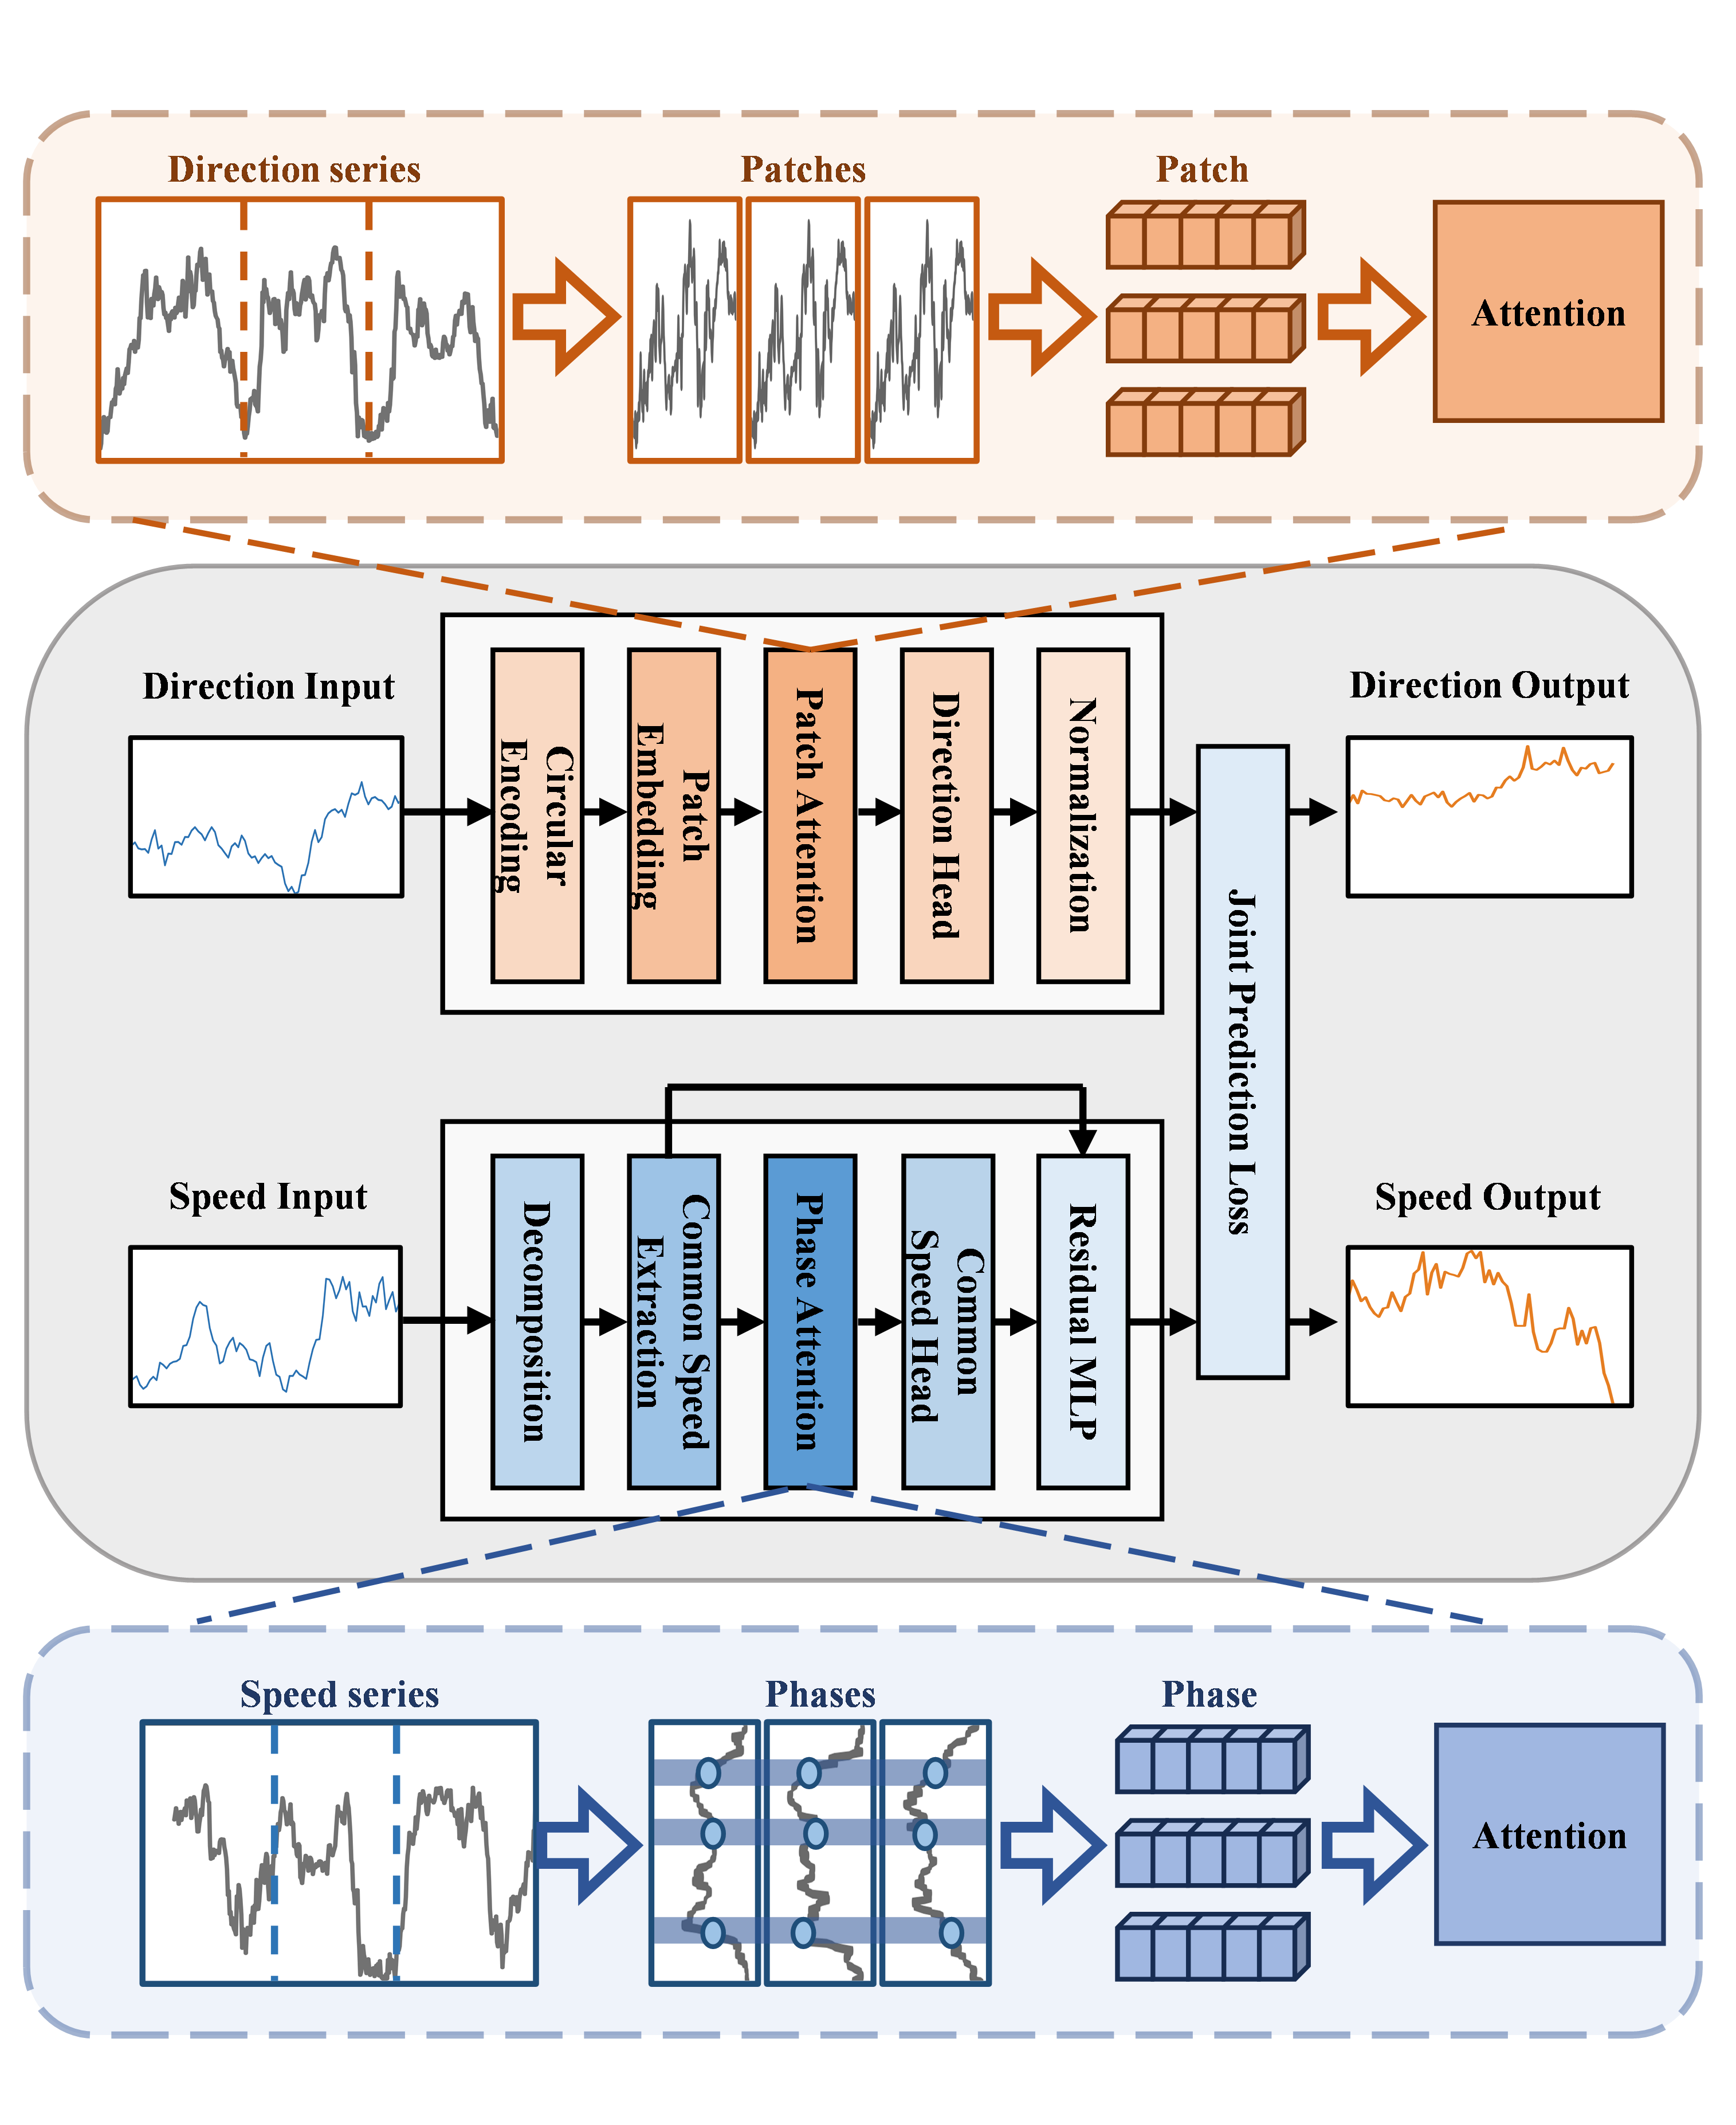
\includegraphics[width=0.5\textwidth]{figures/cscd_architecture.png}
\caption{Overall architecture of WindFormer. The wind speed branch extracts and forecasts common wind speed dynamics with Phase-Attention and restores turbine-level residuals, while the wind direction branch preserves turbine-wise two-dimensional direction sequences through shared Patch-Attention encoding.}
	\label{fig:cscd_architecture}
\end{figure}

\subsection{Overall Model Structure}

The proposed WindFormer is designed around two physical properties of wind farms: wind speeds tend to share common meteorological evolution across turbines, whereas wind directions are recorded as one-dimensional angles and exhibit stronger turbine-specific patterns. As shown in Fig.~\ref{fig:cscd_architecture}, WindFormer contains a wind-speed branch and a wind-direction branch, and the two branches are trained jointly.

Given an input window, the wind-speed branch decomposes the multi-turbine speed field into a common speed component and turbine-level residual components. The common component is encoded by Phase-Attention to capture phase-aligned cross-period evolution, while the residual components are predicted by a shared residual MLP to recover local deviations. The predicted common speed and turbine residuals are then reconstructed into future turbine-wise wind speeds.

The wind-direction branch maps one-dimensional direction angles into two-dimensional sine-cosine unit vectors. For each turbine, the historical two-dimensional direction sequence is partitioned into temporal patches, embedded as patch tokens, and processed by a shared Patch-Attention encoder. A direction prediction head outputs future direction components, which are normalized to unit length before being converted back to angles. This branch preserves turbine-wise directional evolution while sharing temporal parameters across turbines.

The two branches output wind speed and wind direction for the same forecasting horizon. A joint objective combines wind-speed error, direction-vector error, and wind-vector consistency, thereby coupling the two physical quantities during training without forcing them into the same representation space.



\subsection{Learnable Common Wind Speed Extraction}

Let the standardized multi-turbine wind speed be:

\begin{equation}
\tilde{\mathbf{v}}_t = \left[ \tilde{v}_{t,1}, \ldots, \tilde{v}_{t,N} \right].
\end{equation}

The model sets a learnable scalar $a_i$ for each turbine and obtains normalized weights through softmax:

\begin{equation}
\boldsymbol{\alpha} = \operatorname{softmax}(\mathbf{a}), \qquad \sum_{i=1}^{N}\alpha_i=1.
\end{equation}

The common wind speed sequence is defined as:

\begin{equation}
c_t = \sum_{i=1}^{N}\alpha_i\tilde{v}_{t,i}.
\end{equation}

The corresponding wind speed residual for the $i$-th turbine is:

\begin{equation}
r_{t,i} = \tilde{v}_{t,i}-c_t.
\end{equation}

This operation compresses shared wind-farm variations into a common sequence, while turbine-specific deviations are handled by the residual branch.

\subsection{Common Wind Speed Phase-Attention}

\textbf{Candidate period folding.}

Let the common wind speed input sequence be:

\begin{equation}
\mathbf{c}_{1:L} = [c_1, c_2, \ldots, c_L].
\end{equation}

For a candidate period $p$, the model organizes the sequence into multiple local period blocks according to the period position. Let:

\begin{equation}
K_p = \left\lceil\frac{L}{p}\right\rceil,
\end{equation}

then after necessary boundary padding, the sequence can be represented as:

\begin{equation}
\mathbf{C}^{(p)} \in \mathbb{R}^{K_p\times p\times 1}.
\end{equation}

Here, $K_p$ represents the number of period blocks contained in the historical window, and $p$ represents the phase position within each period block. Each period block is flattened into a token:

\begin{equation}
\mathbf{q}^{(p)}_k = \operatorname{Flatten} \left( \mathbf{C}^{(p)}_{k,:,:} \right) \in \mathbb{R}^{p}.
\end{equation}

For multiple candidate periods collected in $\mathcal{P}$, the model organizes short-term temporal patterns at different phase scales.

\textbf{Router-based Phase Attention.}

Each phase token first undergoes linear projection to obtain a $d_m$-dimensional representation, and learnable position encoding is added:

\begin{equation}
\mathbf{e}^{(p)}_k = \operatorname{LN} \left( \mathbf{W}_{\mathrm{in}}^{(p)} \mathbf{q}^{(p)}_k \right) + \mathbf{p}^{(p)}_k.
\end{equation}

To aggregate context across different period blocks, the model introduces $R$ learnable router tokens. Let:

\begin{equation}
\mathbf{R}^{(p)} \in \mathbb{R}^{R\times d_m},
\end{equation}

then the routers first extract global information from the period tokens:

\begin{equation}
\mathbf{C}^{(p)} = \operatorname{Attn} \left( \mathbf{R}^{(p)}, \mathbf{E}^{(p)}, \mathbf{E}^{(p)} \right),
\end{equation}

Subsequently, the period tokens read the cross-period context from the router representations:

\begin{equation}
\widetilde{\mathbf{E}}^{(p)} = \operatorname{Attn} \left( \mathbf{E}^{(p)}, \mathbf{C}^{(p)}, \mathbf{C}^{(p)} \right).
\end{equation}

With residual connections, layer normalization, and feed-forward networks, router tokens summarize cross-period context without full pairwise interaction among all period tokens.

\textbf{Multi-scale common wind speed prediction.}

For each candidate period, the model concatenates the last period token with the average representation of all period tokens:

\begin{equation}
\mathbf{s}^{(p)} = \left[ \widetilde{\mathbf{e}}^{(p)}_{K_p}; \frac{1}{K_p} \sum_{k=1}^{K_p} \widetilde{\mathbf{e}}^{(p)}_k \right].
\end{equation}

Subsequently, the future common wind speed is obtained through the period branch prediction head:

\begin{equation}
\hat{\mathbf{c}}^{(p)} = f_{\mathrm{head}}^{(p)} \left( \mathbf{s}^{(p)} \right) \in \mathbb{R}^{H}.
\end{equation}

The prediction results of different candidate periods are combined by learnable period fusion weights:

\begin{equation}
\hat{\mathbf{c}} = \sum_{p\in\mathcal{P}} \beta_p\hat{\mathbf{c}}^{(p)}, \qquad \beta_p = \frac{\exp(\gamma_p)}{\sum_{q\in\mathcal{P}}\exp(\gamma_q)}.
\end{equation}

Thus, Phase-Attention learns a fusion of multiple short-term candidate scales rather than relying on a single fixed period.

\subsection{Shared Wind Speed Residual Prediction and Reconstruction}

Common wind speed prediction describes shared farm-level variation, while turbine-level residuals recover local dynamics. For the $i$-th turbine, the residual historical sequence is:

\begin{equation}
\mathbf{r}_i = [r_{1,i}, r_{2,i}, \ldots, r_{L,i}].
\end{equation}

The residual branch uses a shared MLP to predict local deviations. Taking the last observed residual $r_{L,i}$ as a reference, the centered sequence is:

\begin{equation}
\widetilde{r}_{t,i} = r_{t,i}-r_{L,i}.
\end{equation}

The shared residual predictor outputs the future residual variation:

\begin{equation}
\Delta\hat{\mathbf{r}}_i = f_{\mathrm{MLP}} \left( \widetilde{\mathbf{r}}_i \right).
\end{equation}

The final residual prediction is:

\begin{equation}
\hat{r}_{h,i} = r_{L,i} + \Delta\hat{r}_{h,i}, \qquad h=1,\ldots,H.
\end{equation}

In the standardized wind speed space, the model uses turbine-level learnable scaling $s_i$ and bias $b_i$ to reconstruct the future wind speed:

\begin{equation}
\hat{\tilde{v}}_{h,i} = s_i\hat{c}_h + b_i + \hat{r}_{h,i}.
\end{equation}

Finally, $\hat{\tilde{v}}_{h,i}$ is unstandardized to obtain the wind speed prediction in the physical space.

\subsection{Wind Direction Independent Patch Transformer}

\textbf{Two-dimensional direction input.}

For the $i$-th turbine, the historical wind direction sequence is represented as:

\begin{equation}
\mathbf{U}_i = \left[ \mathbf{u}_{1,i}, \mathbf{u}_{2,i}, \ldots, \mathbf{u}_{L,i} \right], \qquad \mathbf{u}_{t,i} = [\cos\theta_{t,i}, \sin\theta_{t,i}].
\end{equation}

Accordingly, the direction branch does not extract a common wind direction or construct an additive ``common direction + direction residual'' decomposition. Each turbine direction sequence is maintained as an independent two-dimensional direction input.

\textbf{Temporal patch partitioning.}

For the $L\times 2$ direction sequence of each turbine, a sliding window with length $P$ and step size $S$ constructs temporal patches. The $m$-th patch is:

\begin{equation}
\mathbf{z}_{m,i} = \operatorname{Flatten} \left( \mathbf{U}_{i,(m-1)S+1:(m-1)S+P} \right) \in \mathbb{R}^{2P}.
\end{equation}

The number of generated patches is:

\begin{equation}
M = \left\lfloor \frac{L-P}{S} \right\rfloor+1.
\end{equation}

Each patch contains the sine and cosine components of $P$ time points and is projected to a $d$-dimensional token with positional encoding:

\begin{equation}
\mathbf{e}_{m,i} = \mathbf{W}_{\mathrm{patch}}\mathbf{z}_{m,i} + \mathbf{p}_m.
\end{equation}

This patch representation captures local turning patterns and longer-range directional evolution.

\textbf{Shared Transformer encoding and prediction.}

During direction encoding, each turbine is treated as an independent two-dimensional direction sequence. Turbines share the same patch projection, positional encoding, and Transformer encoder, without token mixing across turbines.

The encoded representation is aggregated using the last patch token and the mean token:

\begin{equation}
\mathbf{h}_i = \left[ \mathbf{e}_{M,i}^{\mathrm{enc}}; \frac{1}{M} \sum_{m=1}^{M} \mathbf{e}_{m,i}^{\mathrm{enc}} \right].
\end{equation}

The prediction head maps $\mathbf{h}_i$ to the two-dimensional direction components for the future $H$ time steps:

\begin{equation}
\hat{\mathbf{U}}_i = f_{\theta}(\mathbf{h}_i) \in \mathbb{R}^{H\times 2}.
\end{equation}

The predicted vectors are L2-normalized before angle recovery:

\begin{equation}
\hat{\mathbf{u}}_{h,i} = \frac{\hat{\mathbf{u}}_{h,i}}{\|\hat{\mathbf{u}}_{h,i}\|_2+\epsilon}.
\end{equation}

Then $\operatorname{atan2}$ recovers the wind direction angle.

\subsection{Joint Loss Function}

\textbf{Wind speed loss.}

Wind speed prediction uses Mean Squared Error in the standardized space:

\begin{equation}
\mathcal{L}_{v} = \operatorname{MSE} \left( \hat{\tilde{\mathbf{V}}}, \tilde{\mathbf{V}} \right).
\end{equation}

\textbf{Direction-vector loss.}

For the predicted direction and true direction, unit vectors are obtained respectively:

\begin{equation}
\hat{\mathbf{u}}_{t,i} = [\hat{u}^{\cos}_{t,i}, \hat{u}^{\sin}_{t,i}], \qquad \mathbf{u}_{t,i} = [u^{\cos}_{t,i}, u^{\sin}_{t,i}].
\end{equation}

The direction error is defined using two-dimensional vector consistency:

\begin{equation}
\ell_{\theta,t,i} = 1 - \hat{\mathbf{u}}_{t,i}^{\mathsf{T}} \mathbf{u}_{t,i}.
\end{equation}

At low wind speeds, wind direction observations are more susceptible to noise; therefore, a reliability weight based on physical wind speed is used:

\begin{equation}
w_{t,i} = \operatorname{clip} \left( \frac{v_{t,i}}{v_0}, 0, 1 \right),
\end{equation}

where $v_0$ is the wind-speed threshold controlling the reliability weight. The weighted direction loss is:

\begin{equation}
\mathcal{L}_{\theta} = \frac{\sum_{t,i}w_{t,i}\ell_{\theta,t,i}}{\sum_{t,i}w_{t,i}+\epsilon}.
\end{equation}

This loss constrains the angle between predicted and true two-dimensional direction vectors and avoids boundary errors from scalar-angle regression.

\textbf{Wind vector consistency loss.}

To constrain speed-direction consistency, physical wind speed is combined with the unit direction vector:

\begin{equation}
\mathbf{q}_{t,i} = v_{t,i} \left[ \cos\theta_{t,i}, \sin\theta_{t,i} \right],
\end{equation}

After scale normalization, predicted and true wind vectors are compared by Smooth L1 loss:

\begin{equation}
\mathcal{L}_{q} = \operatorname{SmoothL1} \left( \frac{\hat{\mathbf{q}}}{\bar{\sigma}_v}, \frac{\mathbf{q}}{\bar{\sigma}_v} \right),
\end{equation}

where $\bar{\sigma}_v$ is the average of the wind speed standard deviations of all turbines.

\textbf{Overall objective.}

The final training objective is:

\begin{equation}
\mathcal{L} = \lambda_v\mathcal{L}_{v} + \lambda_\theta\mathcal{L}_{\theta} + \lambda_q\mathcal{L}_{q}.
\end{equation}

The coefficients balance the wind-speed objective, the direction-vector objective, and the auxiliary wind-vector consistency constraint.
